\chapter{Instruments}
\label{chapter:instruments}

In the following chapters I present data and results from a variety of configurations of two massively redundant low frequency interferometers, PAPER and HERA. In this Chapter I describe these instruments (Section~\ref{sec:used_in_this_work}), along with other current and future low frequency interferometers contributing to EoR science (Section~\ref{sec:not_used_in_this_work}).

\section{Instruments used in this work}
\label{sec:used_in_this_work}

The vision of Hydrogen Epoch of Reionization Arrays was first laid out in the \cite{HERAWhitePaper} White Paper. That work proposed three consecutive efforts, improving upon their predecessors, to construct low frequency interferometers capable of detecting the EoR. While the physical feeds and elements of low frequency interferometers were relatively simple to construct, signal processing, calibration and imaging required new hardware and software to be invented. A research community of observational cosmologists interested in cosmological {\sc hi} had to be nurtured.

The first of the three stages of Reionization Arrays was a parallel effort. The Precision Array for Probing the Epoch of Reionization (PAPER; Section~\ref{subsec:paper_instrument}) and the Murchinson Widefield Array (MWA; Section~\ref{subsec:mwa_instrument}) investigated separate approaches to\footnote{Among other things, see Section III B of \citet{HERAWhitePaper} for an enumerated list.} antenna design, array layout and calibration techniques, with the objective of setting upper limits on and perhaps detecting the power spectrum of the EoR.

The second stage of the Reionization Arrays brought together the teams from the first stage to design and construct a new interferometer based on the lessons learned from PAPER and the MWA. This new instrument, named \textit{the} Hydrogen Epoch of Reionization Array (HERA; Section~\ref{subsec:hera_instrument}) is currently under construction with a build-out schedule that brings new antennas online as they are commissioned. HERA's objective is not only the detection of the EoR power spectrum, but its characterization at very high signal-to-noise. Attempts at low-fidelity imaging of ionized bubbles will be made.

The nature of the third stage is, at the time of writing, somewhat undetermined and contingent on the next decade of funding for low frequency radio astronomy ({\color{red}CITE CITE CITE}). In the vision of \cite{HERAWhitePaper}, its objective will be to image structure evolution throughout the EoR.

\subsection{The Donald C. Backer Precision Array for Probing the Epoch of Reionization (PAPER)}
\label{subsec:paper_instrument}

Much of this thesis presents data from PAPER. PAPER was planned, like HERA, as a staged build-out to larger and larger arrays. In each build-out the correlator was replaced, and (nominally) identical antennae and signal chains were added to the existing array. The first iterations of PAPER consisted of 8 dipole antennae in Green Bank, West Virginia and 4 in Western Australia \citep{Parsons.10}. While the Australian site had a far better observing environment in terms of human-generated radio interference, the site in the USA was easier for the team to design and test on ({\color{red} check with James}). The array in Green Bank was build-up to 32 antennae \citep{Pober.12} and reconfigured from a more traditional ``imaging" configuration to a redundant grid \citep{Parsons.12b}, in order to experiment with redundant calibration and increased sensitivity to discrete Fourier modes. 

While the PAPER-32 array was under operation in Green Bank it became clear that the radio frequency interference (RFI) environment was bad enough to inhibit the science goals of the experiment. ({\color{red} check with James about history of move to SA}).

\subsubsection{The PAPER signal chain}

\subsubsection{PAPER-32}

The PAPER-32 array in South Africa used a highly redundant configuration in order to take the measurements resulting in, at the time, the strongest upper limits on the EoR power spectrum \citep[][sections of \citet{Moore.17} are presented in Chapter~\ref{chapter:ionosphere}]{Parsons.14, Jacobs.15, Moore.17}. The array was in redundant configuration from December 2011 to February 2012. For three nights in September 2011, the 32 elements were reconfigured into an polarized imaging configuration. The results from this deployment were used to make the first 2D power spectra of polarization, presented in \cite{Kohn.16} and in Chapter~\ref{chapter:eor_window_paper32img}. For images and a brief description, see Figure~\ref{fig:instruments_psa32layout}.

\begin{figure}
\centering
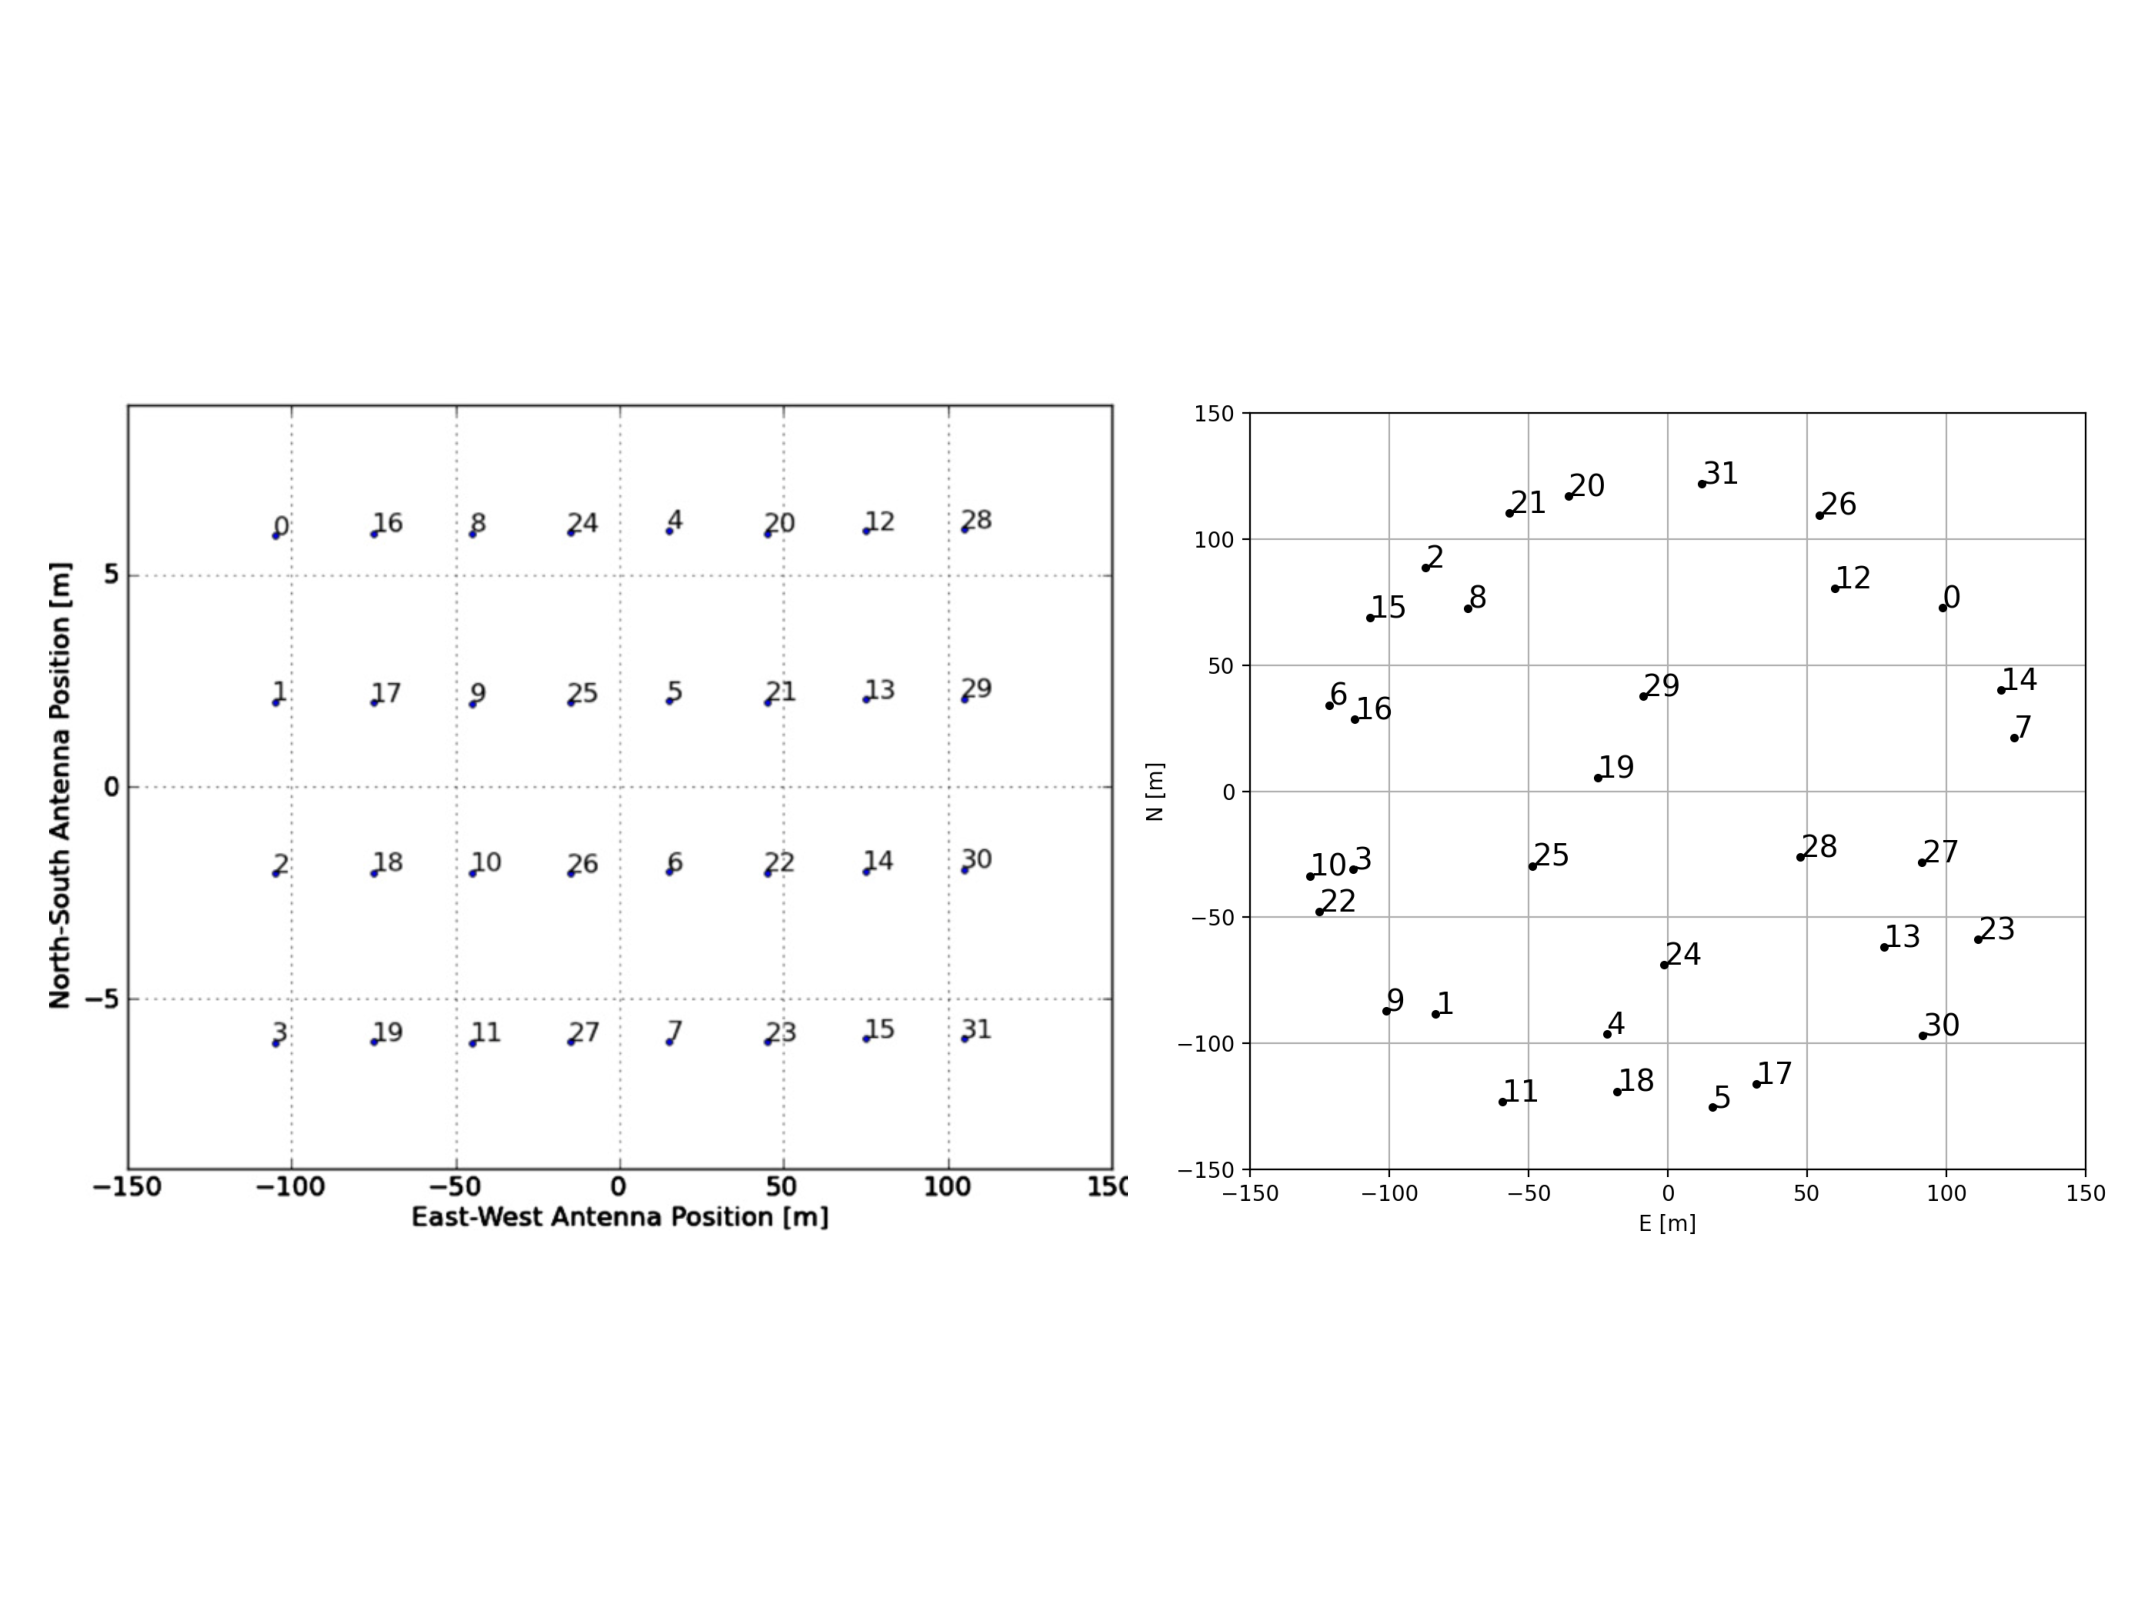
\includegraphics[width=0.9\textwidth]{chapters/instruments/figures/psa32_layouts.pdf}
\caption[The array layouts of the PAPER-32 element deployment in South Africa.]{The array layouts of the PAPER-32 element deployment in South Africa. \textit{Left}: The redundant grid. Four rows, with each element 30\,m from the next in the East-West direction, and closely-packed ($\sim$4\,m) in the North-South direction. Figure taken from \cite{Parsons.14}. \textit{Right}: The polarized imaging array. Elements were arranged in a pseudo-random scatter.}
\label{fig:instruments_psa32layout}
\end{figure}

\subsubsection{PAPER-64}

During the PAPER-32 EoR integration, there were actually 64 antennas present in the Karoo, South Africa. However, the correlator at that time could only process 64 voltage streams -- enough for 32 dual-polarization antennae. This is why 64 element single-instrument-polarization imaging results were published prior to any PAPER-32 studies \citep{Jacobs.13, Stefan.13}. EoR integrations in the 64 element redundant configuration were only possible after a new correlator was produced in 2012. Results from this array were published in \cite[][{\color{red}Cheng et al. \textit{in prep.}, Kolopanis et al. \textit{in prep.}}]{Ali.15, Pober.15}. Diagnostic results from the PAPER-64 redundant configuration that informed studies of time-averaged visibilities are presented in Chapter~\ref{chapter:TAV}. The array layouts are shown in Figure~\ref{fig:instruments_psa64layout}.

\begin{figure}
\centering
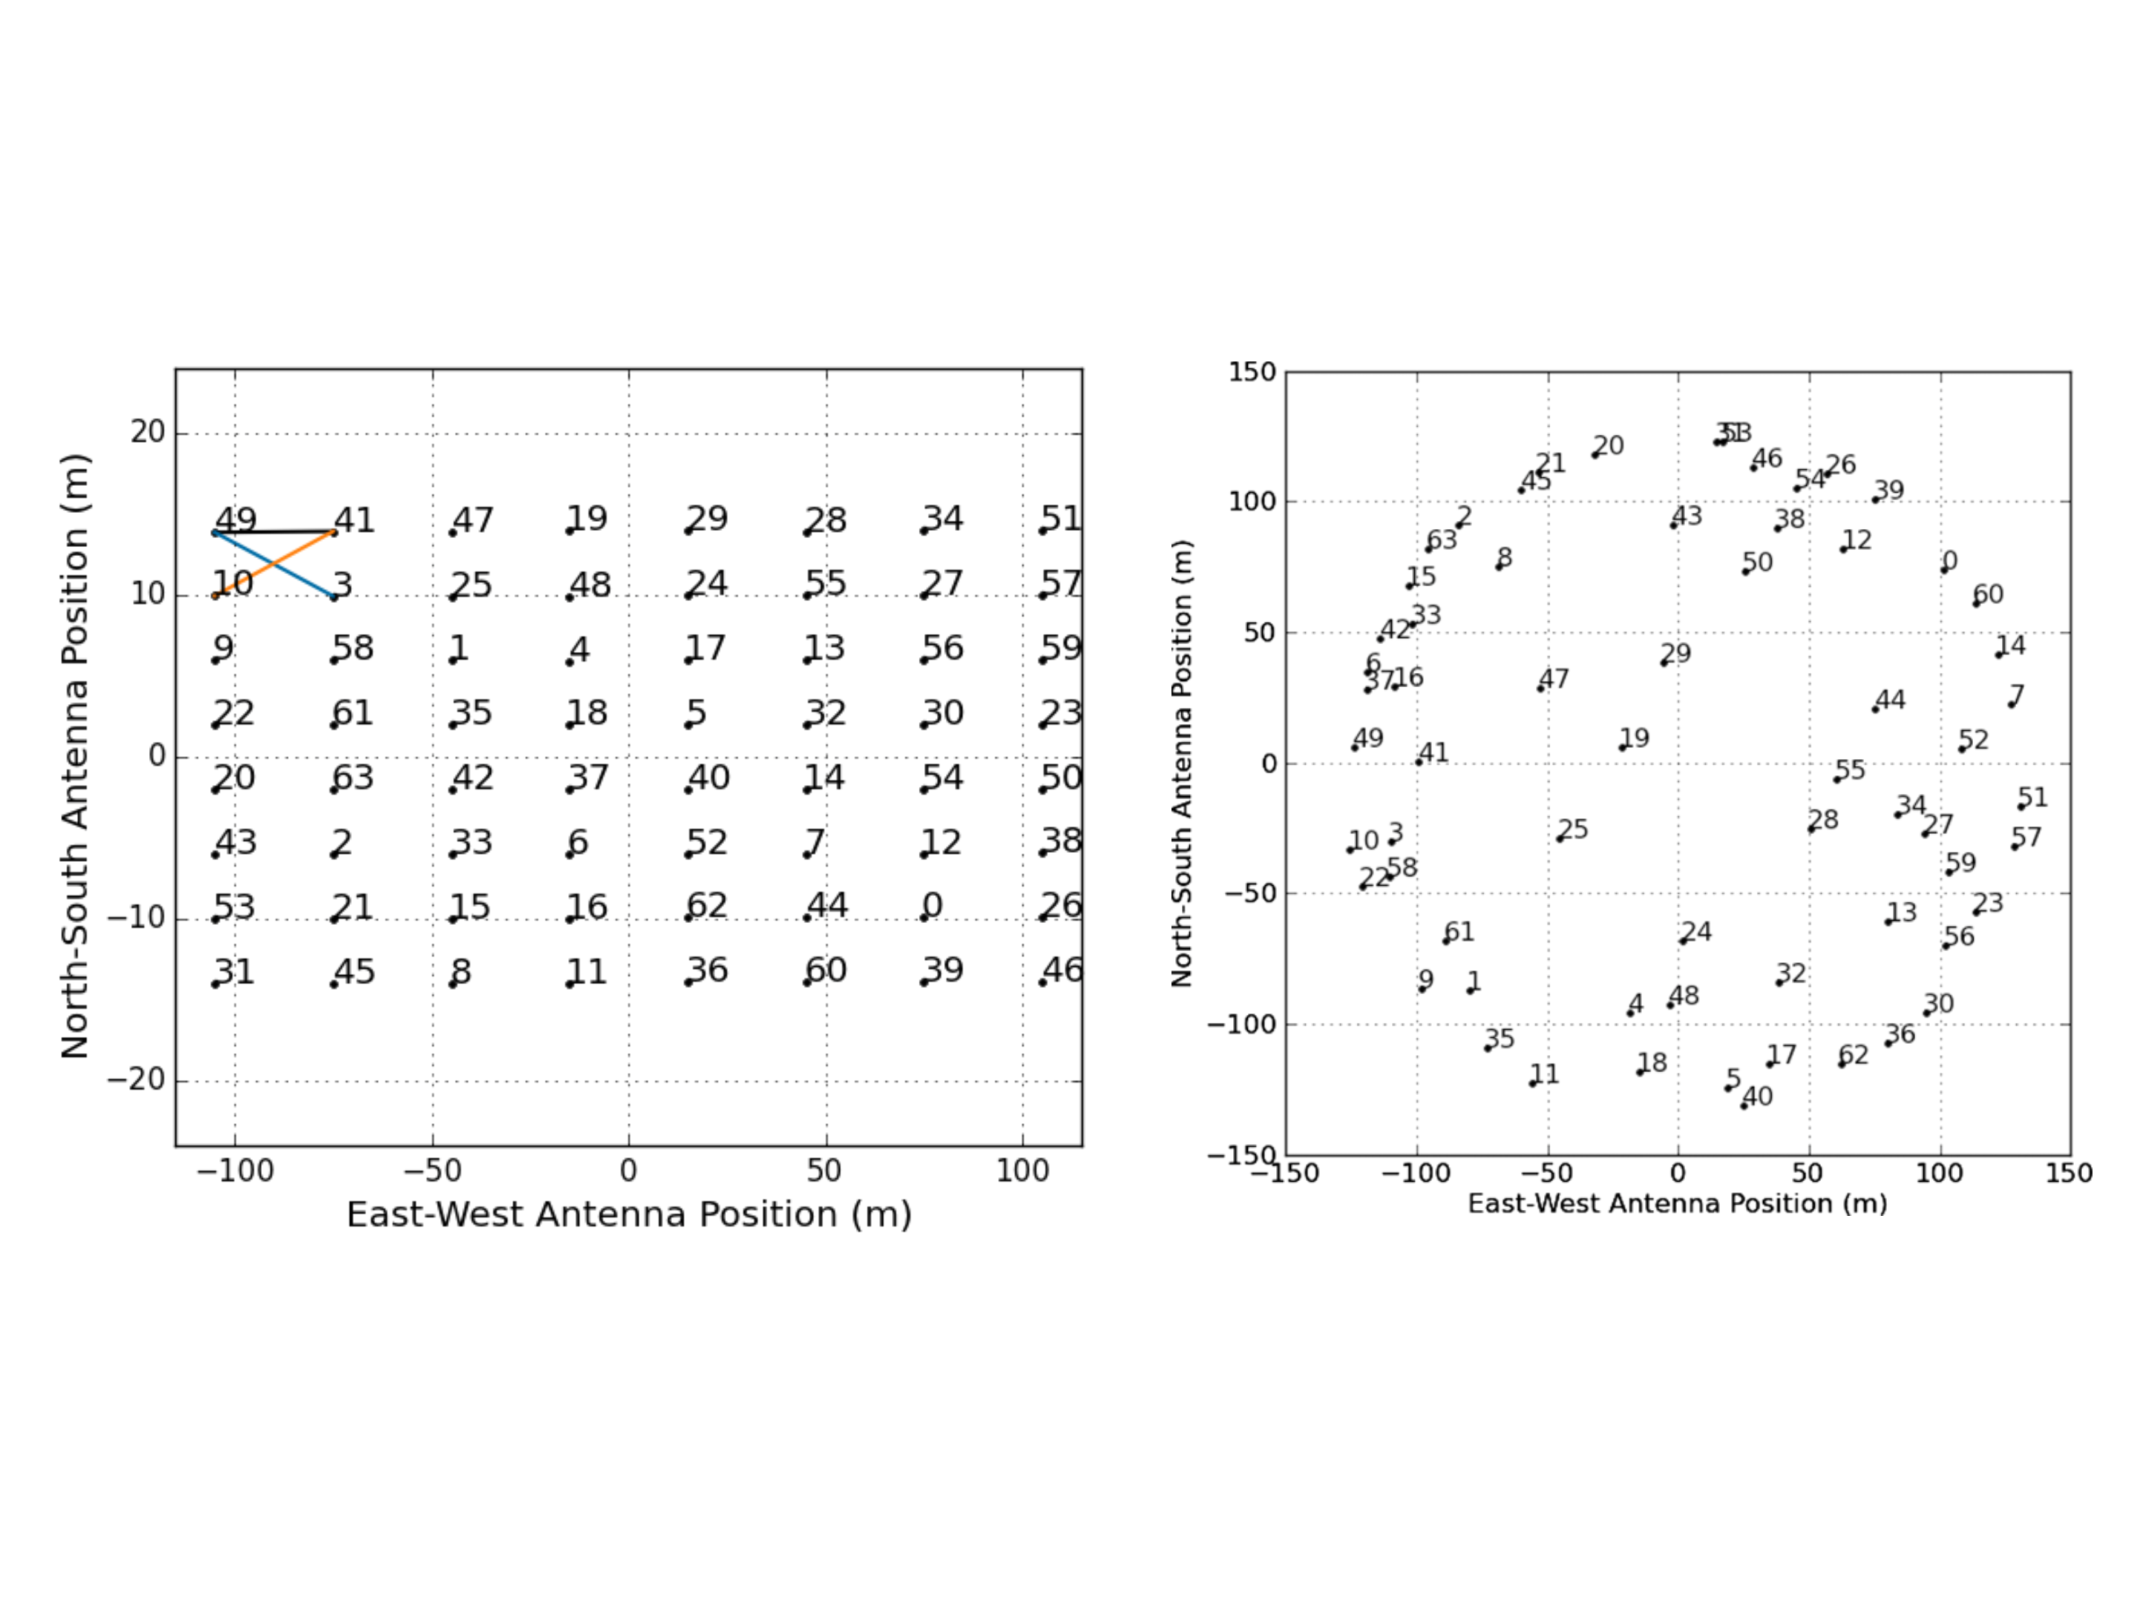
\includegraphics[scale=0.9\textwidth]{chapters/instruments/figures/psa64_layouts.pdf}
\caption[The array layouts of the PAPER-64 deployment.]{The array layouts of the PAPER-64 deployment. \textit{Left}: The redundant grid, built-out from the PAPER-32 grid. Figure taken from \cite{Ali.15}, which highlights the baseline-types used for power spectrum measurements. \textit{Right}: the imaging array, used by \cite{Jacobs.13} to set an absolute flux scale for PAPER experiments. Figure taken from \cite{Jacobs.13}.}
\label{fig:instruments_psa64layout}
\end{figure}

\subsubsection{PAPER-128}

The culmination of the PAPER experiment was the 128 element deployment. There were two observing seasons recorded: November 2013 to March 2014, and July 2014 to January 2015. In this configuration, 112 antennas were laid-out in a redundant grid with 15\,m East-West spacings and 4\,m North-South spacings. The remaining 16 antennas were arranged in `out-rigger' and `in-rigger' positions to increase \textit{uv}-coverage and enable some level of imaging. Results from the first observing season of this array are presented in Chapters~\ref{chapter:data_prep_and_proc}, \ref{chapter:polcal} and \ref{chapter:psa128}. The array layout is shown in Figure

\begin{figure}
\centering
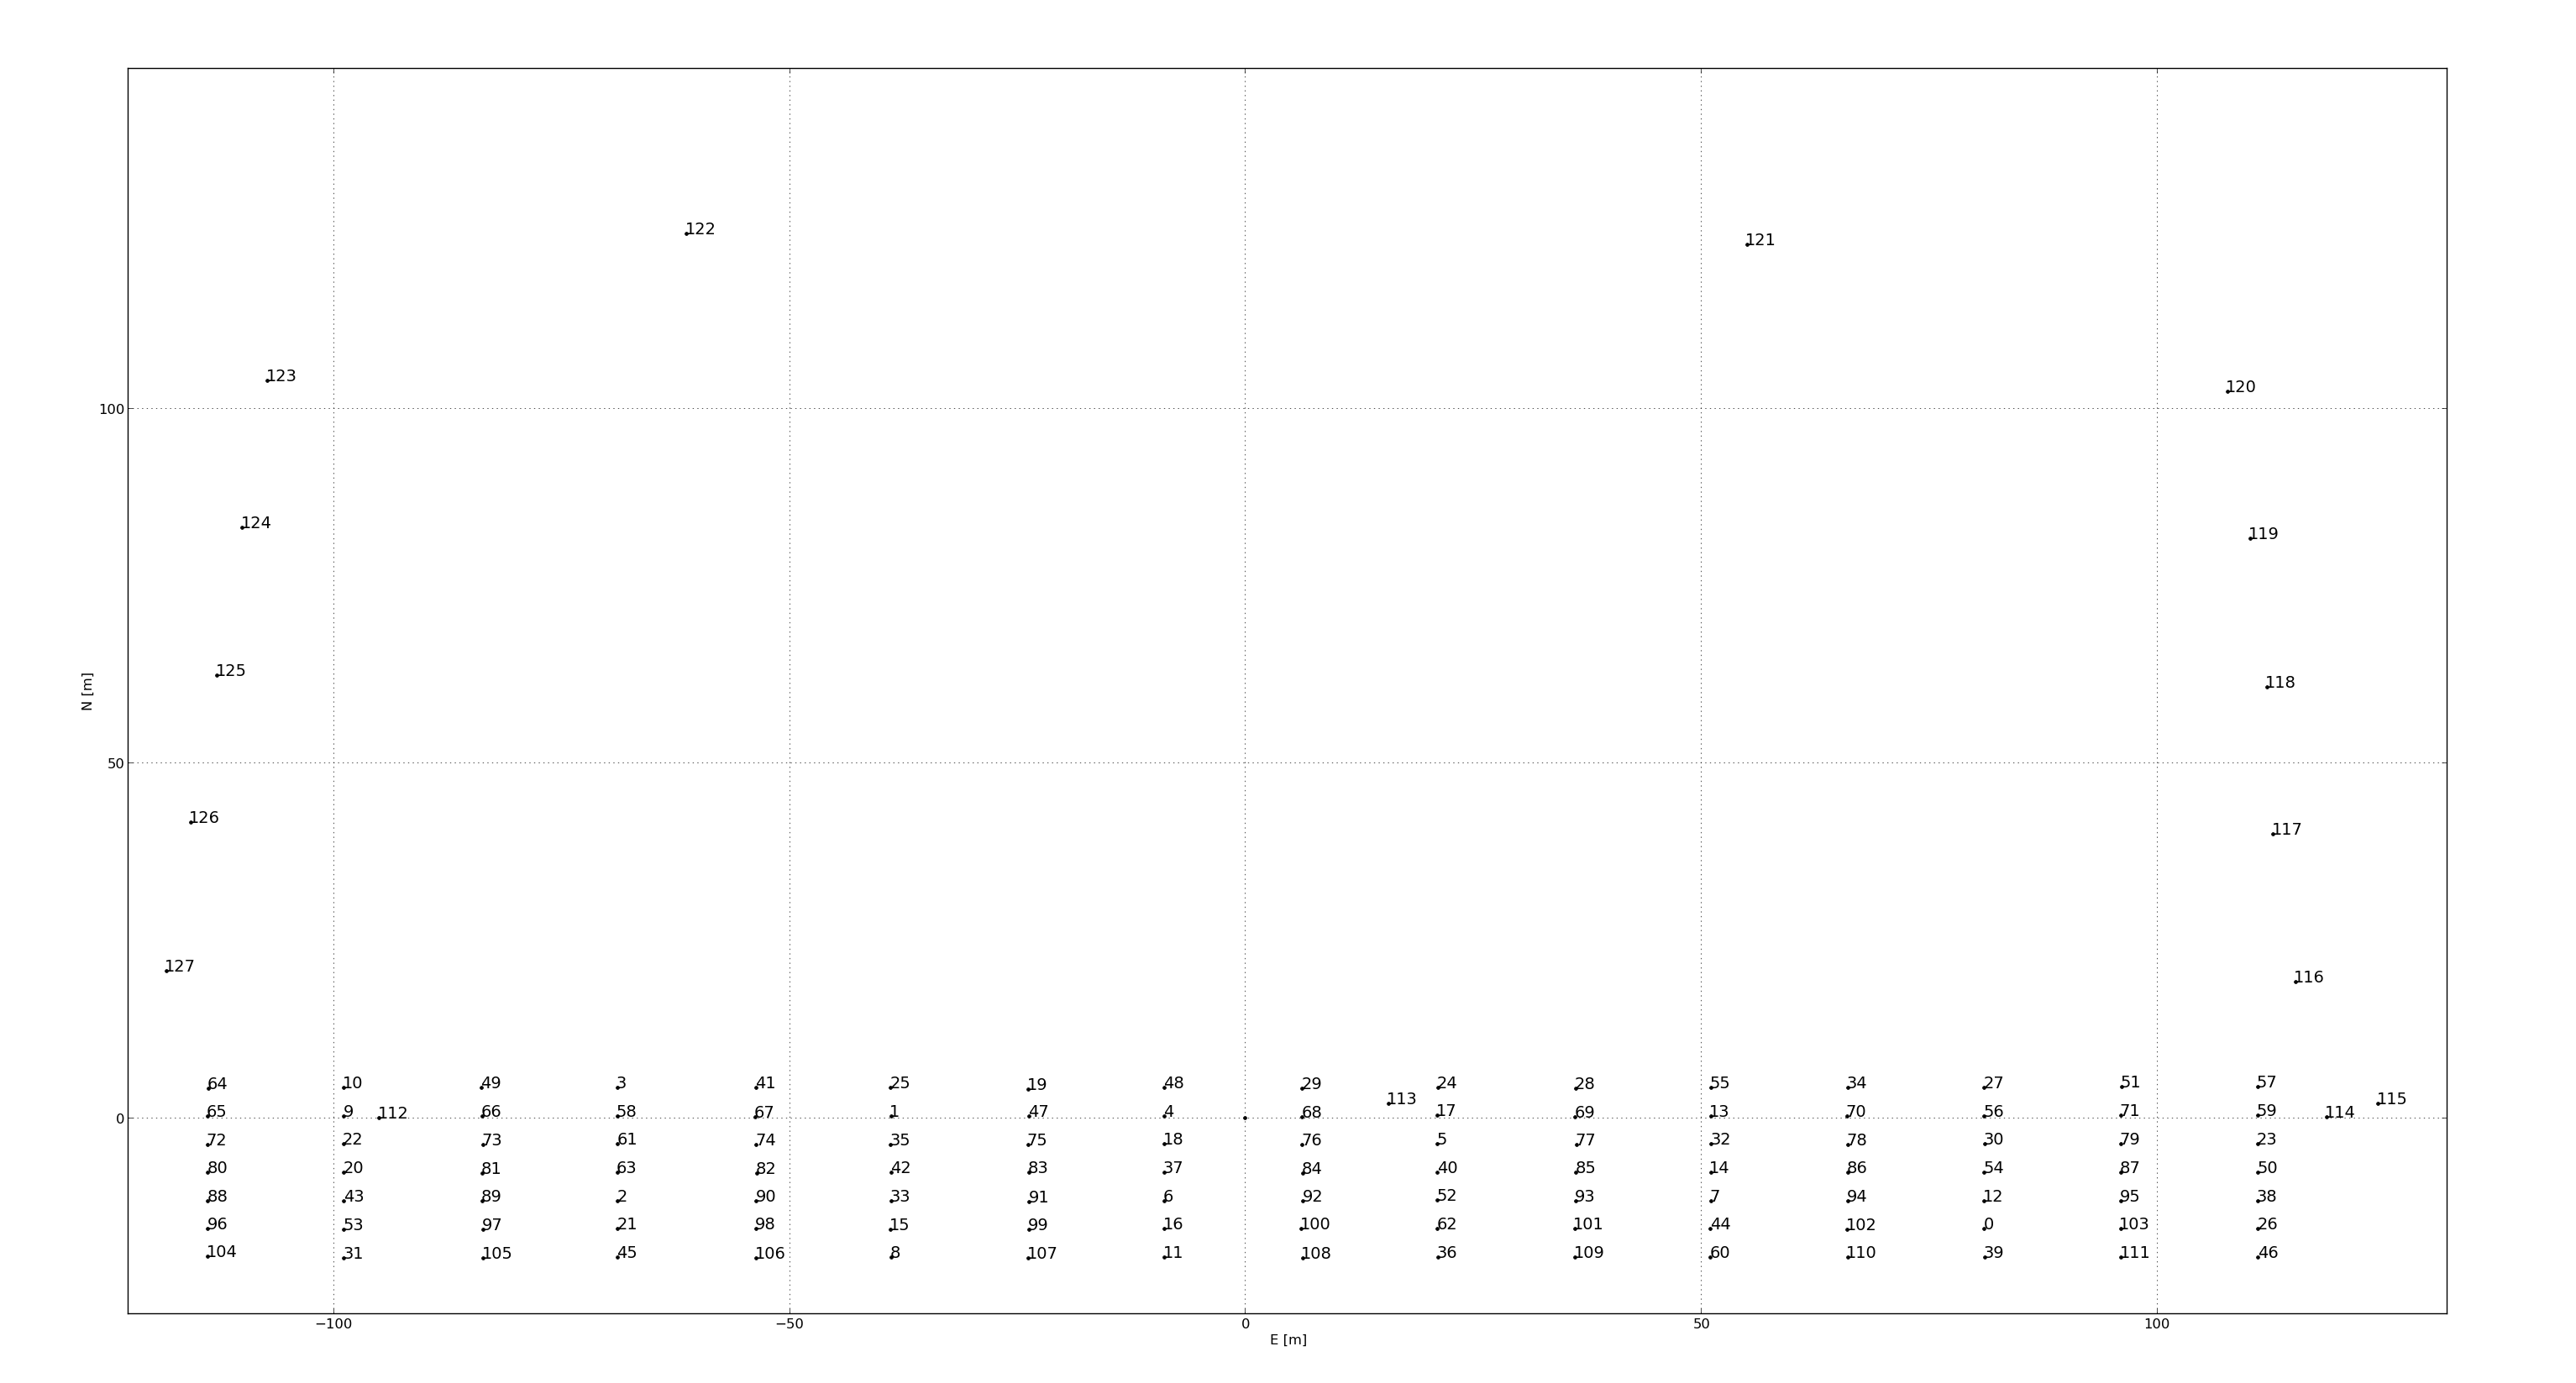
\includegraphics[width=0.9\textwidth]{antlayout_psa128.png}
\caption[The PAPER-128 array layout.]{The PAPER-128 array layout. 112 antennas were laid-out in a redundant grid with 15\,m East-West spacings and 4\,m North-South spacings, and the remaining 16 antennas were arranged in `out-rigger' and `in-rigger' positions to increase \textit{uv}-coverage.}
\end{figure}

\subsection{The Hydrogen Epoch of Reionization Array (HERA)}
\label{subsec:hera_instrument}



\subsubsection{HERA-19 Commissioning Array}
\subsubsection{HERA-47}
\subsubsection{Future HERA Build-Outs}

\section{Other current and future low-frequency interferometers}
\label{sec:not_used_in_this_work}

\subsection{The Low Frequency Array (LOFAR)}
\subsection{The Murchinson Widefield Array (MWA)}
\label{subsec:mwa_instrument}

\subsection{Square Kilometer Array -- Low band (SKA-Low)}
\label{subsec:skalow_instrument}

